%
% Шаблон для НИР
%

\documentclass[a4paper,12pt]{article}
\usepackage[backend=biber,sorting=none]{biblatex} % библиография
\usepackage{mathtext} %русские буквы в формулах
\usepackage[T2A]{fontenc}
\usepackage[utf8]{inputenc}
\usepackage[russian]{babel}
\usepackage{amsmath}
\usepackage{fancyvrb}
\usepackage{formular}
\usepackage{setspace} % управление междустрочными интервалами
%поля документа
\usepackage[left=3cm,right=1cm,top=2cm,bottom=2cm]{geometry}

\usepackage{misccorr} % точки в конце номеров разделов, использовать перед пакетом ccaption!
\usepackage{ccaption} % изменения подписей к рисункам и табл.
% отступ перед первым абзацем
\usepackage{indentfirst}
%вставка изображений
\usepackage{graphicx}
% счетчики
\usepackage{totcount}
% управление содержанием
\usepackage{tocloft}
% управление таблицами и рисунками
\usepackage{float}
\usepackage{tabularx}

%для добавления количества источников в реферат
\newtotcounter{citnum} %From the package documentation
\def\oldbibitem{} \let\oldbibitem=\bibitem
\def\bibitem{\stepcounter{citnum}\oldbibitem}

% окружение для листингов - с нумерацией строк слева
\DefineVerbatimEnvironment{MyCode}{Verbatim}{frame=lines,numbers=left,numberblanklines=false,framesep=5mm}

% автоматическая нумерация листингов
\newfloat{Program}{phb}{lop}
\floatname{Program}{Листинг}
\floatstyle{ruled}

\setcounter{secnumdepth}{3} % глубина нумерации до подразделов

%если нужны точки в оглавлении для разделов - раскомментируйте следующую команду
%\renewcommand{\cftsecleader}{\cftdotfill{\cftdotsep}}

\addto\captionsrussian{
\renewcommand{\figurename}{Рисунок}
\renewcommand{\tablename}{Таблица}
}

% дефис в подписи к рисункам
\captiondelim{ -- } 

% Настройки для окружений с подчеркиваниями для подписей и пр.
\setFRMfontencoding{T2A}
\setFRMdfontencoding{T2A}
% thanks to A.Starikov
\setFRMfontfamily{cmr}
\setFRMdfontfamily{ptm}
\setFRMdfontsize{10pt}

% задает длину поля для подписи на титульной странице
\newFRMfield{xtitlesign}{40mm}

% поле для факультета или кафедры
\newFRMfield{fcath}{65mm}


\addbibresource{rbiblio.bib}

\begin{document}

% счетчики страниц, рисунков, таблиц
\regtotcounter{page}
\regtotcounter{figure}
\regtotcounter{table}

\renewcommand{\refname}{\centerline{СПИСОК ИСПОЛЬЗОВАННОЙ ЛИТЕРАТУРЫ}} 
\renewcommand{\contentsname}{\centerline{СОДЕРЖАНИЕ}} 
%\renewcommand{\refname}{Список источников}  % По умолчанию "Список литературы" (article)
%\renewcommand{\bibname}{Литература}  % По умолчанию "Литература" (book и report)

% титульная страница
\thispagestyle{empty}
\begin{center} \small
\textbf{МИНИСТЕРСТВО ОБРАЗОВАНИЯ И НАУКИ РОССИЙСКОЙ ФЕДЕРАЦИИ}\\
ФЕДЕРАЛЬНОЕ ГОСУДАРСТВЕННОЕ АВТОНОМНОЕ ОБРАЗОВАТЕЛЬНОЕ УЧРЕЖДЕНИЕ
ВЫСШЕГО  ОБРАЗОВАНИЯ\\
«Национальный исследовательский ядерный университет «МИФИ»\\
\textbf{Обнинский институт атомной энергетики} – \\
филиал федерального государственного автономного образовательного учреждения высшего\\
образования «Национальный исследовательский ядерный университет «МИФИ»\\
(ИАТЭ НИЯУ МИФИ)
\end{center}
\vfill
\medskip

% Направление подготовки следует уточнять,
% магистры и бакалавры могут иметь разные наименования
\begin{center}
\begin{tabular}{rl}
Отделение & \useFRMfield{fcath}[\large Интеллектуальных кибернетических систем] \\ 
Направление подготовки & \useFRMfield{fcath}[\large Информационные системы и технологии] \\ 
\end{tabular} 
\end{center}

\vfill

\large 

\begin{center}
	Научно-исследовательская работа \\
	
	\medskip
	
	\textbf{\Large 
		Построение системы учета семейного бюджета с использованием QT Framework
	}
	
\end{center}

\vspace{1cm}

\begin{tabular*}{\textwidth}{lcr}
Студент группы ИС-Б14-З & \useFRMfield{xtitlesign} & А.В. Миронов\\
& & \\
Руководитель & & \\
к.т.н., доцент & \useFRMfield{xtitlesign} & О.А. Мирзеабасов
\end{tabular*}


\vfill
\large

\begin{center}
Обнинск, 2018
\end{center}

\onehalfspacing

\pagebreak

% реферат 
\thispagestyle{empty}

\section*{\centering РЕФЕРАТ}

% возможно, кол-во источников придется вставлять вручную
\total{page} стр., \total{table} табл., \total{figure} рис. , \total{citnum} ист. 

\pagebreak
\thispagestyle{empty}


\section*{\centering ОБОЗНАЧЕНИЯ И СОКРАЩЕНИЯ}


\pagebreak



\tableofcontents
% если нужно добавить "Стр." над номерами страниц - раскомментируйте следующую команду
%\addtocontents{toc}{~\hfill\textbf{Стр.}\par}

\pagebreak

\section*{\centering ВВЕДЕНИЕ}
\addcontentsline{toc}{section}{ВВЕДЕНИЕ}
Учет семейного бюджета финансов с каждым годом приобретает все большую значимость для успешного выживания в условиях нашей страны. Конечно существует множество способов выполнить эту задачу, начиная с простой
записи доходов и расходов в тетради и заканчивая сложными програмными
комплексами, позволябщие автоматизировать этот процесс. Среди програмных комплексов широко известны такие как \textbf{GNUCash} или \textbf{Easy Finance}

но по ряду причин таких как, избыточный для меня функционал, и общая сложность контроля, я решил разработать своё приложение, которое сильно облегчит мне эту нелегкую задачу.
Задачи, решаемые в ходе работы:
\begin{enumerate}
\item Формирование идеи приложения
\item Обоснование необходимости разработки
\item Разработка технического задания
\item Подготовка функционального базового прототипа
\item Расширение функционала в соответствии с техническим заданием
\item Создание документации для проекта: Руководство оператора, Руководство программиста
\item Подготовка отчета. 
\end{enumerate}
 % текст введения в файле intro.tex
\pagebreak

%\input{Post_zad}
\pagebreak
% первая глава

\section{Название первого раздела}

\subsection{Подраздел}

Текст подраздела

\subsection{Вставка изображения}

\begin{figure}
	\centering
	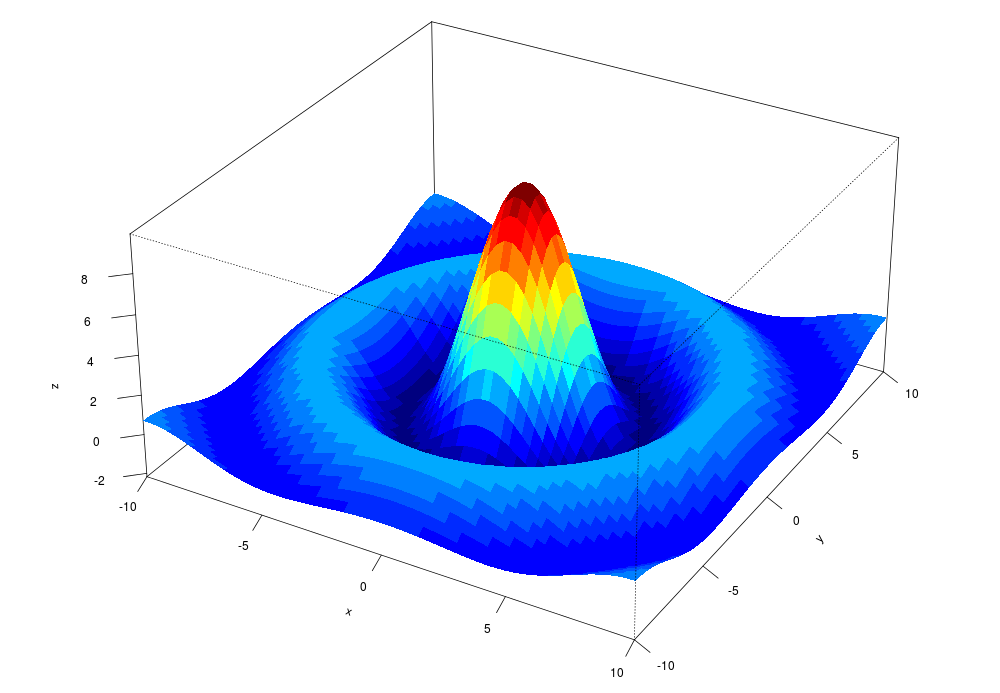
\includegraphics[width=0.7\linewidth]{pics/pic3D}
	\caption{Пример изображения для демонстрации возможности вставки в документ}
	\label{fig:pic3d}
\end{figure}



Изображение на рис.~\ref{fig:pic3d} находится в подкаталоге pics.

  % первая глава - в файле part1.tex
\pagebreak
\part{Техническое задание на разработку программного обеспечения }

\section{Общие положения}
\subsection{Наименование программы}
Наименование программы: «Программа учёта персональных финансов Snipe Studio Budget Manager».
\subsection{Назначение и область применения}
Программа предназначена для учета домашних финансов и личных средств и не может быть применена для ведения бухгалтерии на предприятиях.
\subsection{Основания для разработки}
Данная программа разрабатывается в рамках постановки задачи от руководителя выпускной квалификационной работы для ИАТЭ НИЯУ МИФИ. 
\section{Требования к программе}
\subsection{Требования к функциональным характеристикам }
Программа должна обеспечивать возможность выполнения перечисленных ниже функций:
\begin{enumerate}
	\item Функции добавления записи в базу данных. Доход и расход должны быть выполнены с использованием отдельных кнопок
	\item Функции изменения записей в базе данных с возможностью изменить тип записи
	\item Функции удаления записей в базе данных без возможности их восстановления
	\item Возможности изменения места хранения лога приложения и базы данных через окно выбора директории
	\item Возможность изменения отображаемой валюты
	\item Возможность изменения локализации для следующих языков: \begin{enumerate}
		\item Русский
		\item Английский
		\item Голландский
		\item Немецкий
		\item Французский
	\end{enumerate}
	\item Возможность изменить уровень логирования вплоть до полного отключения записи логов
	\item Функцию полной очистки базы данных без возможности восстановления
	\item Функцию экспорта данных из программы в согласованом формате
	\item Функцию импорта данных в программу из файла, записанного в согласованном формате
	\item Возможность комфортной работы в полноэкранном режиме (при развороте приложения)
	\item Функцию работы с горячими клавишами	
\end{enumerate}

\subsection{Требования к организации входных данных}
Данные для работы программы предварительно не требуется организовывать. Исключение составляет только функция импорта. Формат экспортируемых и импортируемых данных:\\
\textit{1-ая строка: количество добавляемых записей\\
2-ая и последующие строки содержат список полей записи разделенных символом «;»\\
1-я позиция — порядковый номер записи, при импорте игнорируется.\\
2-я позиция — дата и время выполнения операции\\
3-я позиция — Сумма операции\\
4-я позиция — Коментарий к операции\\
5-я позиция — не используется\\
6-я позиция — Тип операции (1 — доход, 0 — расход)}

Тип файла для импорта должен соответствовать текстовому файлу (csv, txt, и.т.п.)\\

Файлы указанного формата должны размещаться (храниться) на локальных или съемных носителях, отформатированным согласно требованиям операционной системы.

\subsection{Требования к организации выходных данных}
См. Требования к организации входных данных\\
\subsection{Требования к временным характеристикам}
Требования к временным характеристикам к программе не предъявляются\\

\subsection{Требования к надежности}
\subsubsection{Требования к обеспечению надежного (устойчивого) функционирования программы}
Надежное (устойчивое) функционирование программы должно быть обеспечено выполнением Заказчиком совокупности операционно-технических мероприятий перечень которых приведен ниже:
\begin{enumerate}
	\item Организацией бесперебойного питания технических средств
\end{enumerate}

\subsubsection{Время восстановления после отказа}
Время восстановления после отказа, вызванного сбоем электропитания технических средств (иными внешними факторами), не фатальным сбоем (не крахом) операционной системы, не должно превышать 15 секунд без учета времени полной загрузки операционной системы.\\

Время восстановления после отказа, вызванного фатальным сбоем (крахом) операционной системы не должно превышать времени, требуемого на устранение неисправностей технических средств и переустановки програмных средств.\\
\subsubsection{Отказы из-за некорректных действий пользователя}
Отказы программы возможны в случае некорректных действий пользователя при взаимодействии с операционной системой. Во избежании возникновения отказов по указанной выше причине следует обеспечить работу конечного пользователя без предоставления ему административных привелегий\\
\section{Условия эксплуатации}
\subsubsection{Климатические условия эксплуатации}
Климатические условия эксплуатации, при которых должны обеспечиваться данные характеристики, должны удовлетворять требованиям, предъявляемым к техническим средствам в части условий их эксплуатации.\\
\section{Требования к видам обслуживания}
Программа не требует проведения каких либо видов обслуживания
\section{Требования к численности и квалификации персонала}
Минимальное количество персонала, требуемого для работы программы, должно составлять не менее 1 штатной единицы — конечный пользователь программы — оператор.\\

Конечный пользователь программы (оператор) должен обладать минимальными навыками работы с графическим пользовательским интерфейсом операционной системы.\\
\section{Требования к составу и параметрам технических средств.}
В состав технических средств должен входить IBM-совместимый персональный компьютер на базе процессоров архитектур x64 или x86 c размером свободной оперативной памяти не менее 50 Мб\\
\section{Требования к информационным структурам и методам решения}
Требования к информационным структурам (файлов) на входе и выходе, а также к методам решения не предъявляются\\

Исходные коды программы должны быть реализованы на языке C++ с расширением QT5. В качестве интегрированной среды разработки программы должна быть использована среда QTCreator.\\
\section{Требования к защите информации и программ}
Требования к защите информации и программ не предъявляется.\\
\section{Требования к маркировке и упаковке.}
Требования к маркировке и упаковке не предъявляется.\\
\section{Специальные требования}
Программа должна обеспечивать взаимодействие с пользователем (оператором) посредством графического интерфейса, согласно рекомендациям компании-производителя операционной системы.\\
\section{Технико-экономические показатели}
Ориентировочная экономическая эффективность не расчитывается\\
Предполагаемое использование программы в год до 2000 сеансов работы в год\\

\section{Стадии и этапы разработки}
\subsection{Стадии разработки}
Разработка должна производится в 2 этапа:
\begin{enumerate}
	\item Разработка технического задания
	\item Рабочее проектирование
\end{enumerate}

Этап внедрения не предполагается, т.к. система не предназначена для использования на предприятиях\\
\subsubsection{Этапы разработки}
На стадии разработки технического задания должен быть выполнен этап разработки, согласования и утверждения настоящего технического задания.\\

На стадии рабочего проектирования должны быть выполнены перечисленные ниже этапы работ:
\begin{enumerate}
	\item Разработка программы
	\item Испытание программы
\end{enumerate}

\subsection{Содержание работы по этапам}
На этапе разработки технического задания должны быть выполнены перечисленные ниже работы:
\begin{enumerate}
\item Постановка задач
\item Определение и уточнение требований к технической документации
\item Определение требований к программе
\item Определение стадий, этапов и сроков разработки программы и документации
\item выбор языка программирования
\item Согласование и утверждение технического задания
\end{enumerate}

На этапе разработки должно быть выполнено кодирование и отладка программы.\\

На этапе испытаний должны быть выполнено проведение приемо-передаточных испытаний и корректировка программы по результатам испытаний.\\
 % вторая глава - в файле part2.tex
\pagebreak
% !TeX spellcheck = de_DE
\part{Выбор инструментов и средств разработки}
\section{Обзор и выбор СУБД}
\subsection{СУБД MySQL}
MySQL — свободная реляционная система управления базами данных. Разработку и поддержку MySQL осуществляет корпорация Oracle, получившая права на торговую марку вместе с поглощённой Sun Microsystems, которая ранее приобрела шведскую компанию MySQL AB. Продукт распространяется как под GNU General Public License, так и под собственной коммерческой лицензией. Помимо этого, разработчики создают функциональность по заказу лицензионных пользователей.\cite{mysql}\\
\subsection{СУБД SQLite}
SQLite — это встраиваемая кроссплатформенная БД, которая поддерживает достаточно полный набор команд SQL и доступна в исходных кодах (на языке C). Исходные коды SQLite находятся в public domain, то есть вообще никаких ограничений на использование.\\
\subsection{Обоснование выбора СУБД}
Для наибольшего удобства была использована SQLite, что позволило достаточно сильно ускорить скорость открытия потребления, а также существенно снизить потребляемое количество оперативной памяти. В ранних версиях программы при наличии большого количества записей в базе данных программа пыталась полностью перенести данные в память, что приводило к общему замедлению работы операционной системы и возможному повреждению данных.

\section{Обзор и выбор языка программирования}
При выборе языка программирования для создания приложения я остановился на трех базовых концепциях:

\begin{enumerate}
	\item Портируемость
	\item Легкость
	\item Удобство использования
	\item Большие возможности
\end{enumerate}

Благодаря этому списку мне удалось достаточно сильно сократить число
языков программирования на которых можно было написать приложение, в
итоге я остановился на языке

C++ с расширением QT Framework. Который оказался достаточно комфортным и легко расширяемым для выполнения необходимых задач.

\part{Разработка базы данных для хранения информации}
\section{Проектирование базы данных}
База данных состоит из 1 таблицы имеющую создающуюся с помощью следующего запроса:
\begin{MyCode}
	CREATE TABLE  IF NOT EXISTS "operations"(
	"id" INTEGER  PRIMARY KEY  NOT NULL ,
	"time" DATETIME DEFAULT (CURRENT_TIMESTAMP),
	"summ" NOT NULL  DEFAULT (null),
	"comment"  NOT NULL,
	"catid" INTEGER DEFAULT (null),
	"side" BOOL DEFAULT (0))
\end{MyCode}

\section{Реализация базы данных в СУБД SQLite}
Таблица создается в базе данных при запуске программы используя запрос указанный выше\\
 % вторая глава - в файле part3.tex


\pagebreak
\section*{\centering ЗАКЛЮЧЕНИЕ}
\addcontentsline{toc}{section}{ЗАКЛЮЧЕНИЕ}
Настоящая научно-исследовательская работа посвящена созданию приложения по ведению домашней бухгалтерии на языке

C++ с расширением QT

Framework. В результате была разработано приложение, позволяющее учитывать расходы и доходы в достаточно удобном интерфейсе.
% оформление библиографии - вариант с БД

\pagebreak
\nocite{qtdoc}
\nocite{qt532015}
\nocite{Warren2007}
\nocite{AzureDevops}
\addcontentsline{toc}{section}{СПИСОК ИСПОЛЬЗОВАННОЙ ЛИТЕРАТУРЫ}
\printbibliography

\pagebreak
\section*{\centering Приложение}
\addcontentsline{toc}{section}{Приложение}


\end{document}          

